\chapter{Validation against morphological simulations} \label{Chp:Morphology}

In 2022, the pilot implementation of the \emph{stepped-hydrograph} approach was tested using two cases for which the \dfastmi results (using steady state flow fields obtained using Delft3D-FLOW) were compared against long-term morphological simulations carried out using Delft3D-FLOW/MOR.
See \citet{GiriJagers2022} for details.
The theory of the \emph{stepped-hydrograph} approach is documented in \citet{JagersGiri2022} and the latest version of the \citet{um}.
At that time a number of different hydrographs were compared.
The hydrograph which is selected for use in \dfmi 3 differs from the ones used in that report.
Therefore, part of that analysis has been repeated here:

\begin{itemize}
\item \nameref{Sec:Palmerswaard}
\item \nameref{Sec:PannerdenschCanal}
\end{itemize}

\section{Palmerswaard} \label{Sec:Palmerswaard}

\emph{The input files of this case are included in the distribution under \file{examples/01 - Palmerswaard}.}

The intervention concerns a secondary channel planned in the "Palmerswaard" which is located along the river Rhine (Nederrijn) at river kilometre (Rkm) 910-912 in the reach upstream of the Amerongen barrier at Rkm 922.
An overview of the intervention is given in \autoref{Palmers_proj}.
This case is included as Example 1 in the \citet{um}.
For this analysis, the Nederrijn grid of the DVR\footnote{Duurzame Vaarweg Rijntakken} model has been used.
The reference model is based on the Baseline schematization 'rijn-beno18\_5-v1a'.
Since the DVR model was too coarse to represent the actual secondary channel, a combination of flow extraction (at Rkm 910.5) and insertion (at Rkm 912) was used to represent the side channel.

We compare the results of \dfmi with the results of a morphological simulation using Delft3D-FLOW.
For consistency with the morphological simulation using Delft3D-FLOW, the \dfmi analysis was performed using steady-state hydrodynamic conditions also obtained using Delft3D-FLOW.

\begin{figure}
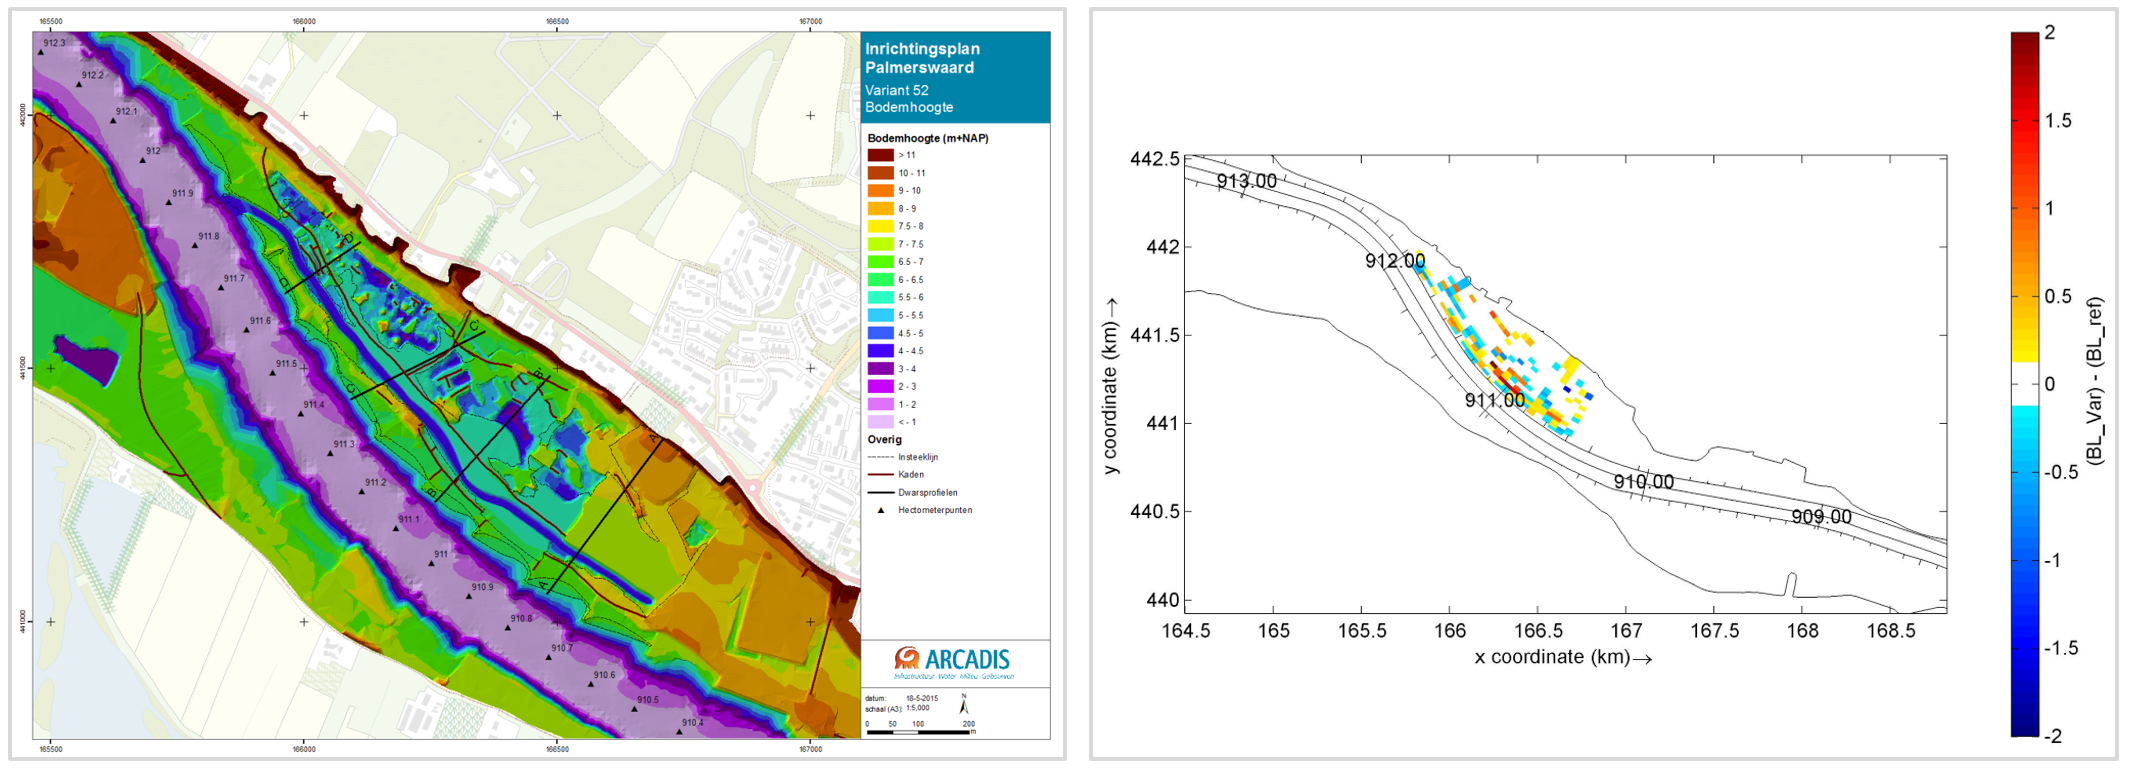
\includegraphics[width=\columnwidth]{figures/Palmerswaard_proj.png}
\caption{Side channel design (left) and initial representation on the grid (right).}
\label{Palmers_proj}
\end{figure}

Since the intervention is located on the Rhine branches, the new \dfmi method requires simulation results for 6 steady discharges: 1300, 2000, 3000, 4000, 6000, and \SI{8000}{\metre\cubed\per\second} at Lobith.
However, since the intervention is located in the backwater curve of the Amerongen barrier which is closed at discharges below \SI{1500}{\metre\cubed\per\second} causing largely stagnant flow conditions, the lowest discharge isn't relevant for this case.

\citet{GiriJagers2022} observed that the morphological impact of this intervention was properly reproduced using a \dfmi analysis using the full set of discharges in the \emph{stepped-hydrograph} of the morphological simulation.
Here we compare the results with the results of the \dfmi analysis using the simplified hydrograph consisting of only the discharges 1300, 2000, 3000, 4000, 6000, and \SI{8000}{\metre\cubed\per\second} at Lobith.

\begin{figure}
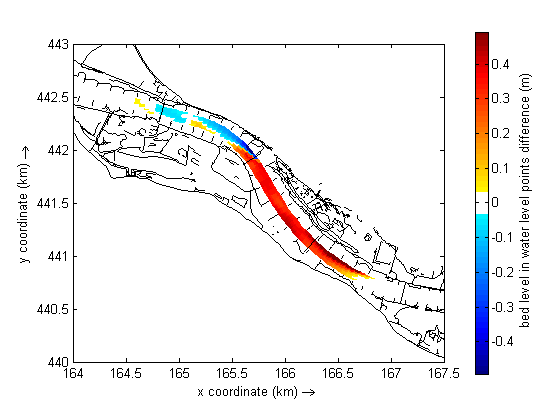
\includegraphics[width=\columnwidth/2]{figures/Palmerswaard_delft3d.png}
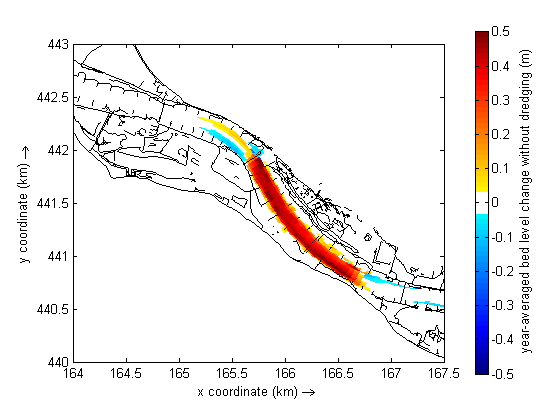
\includegraphics[width=\columnwidth/2]{figures/Palmerswaard_dfastmi.png}
%\fbox{\parbox{\columnwidth}{\todo{Results to be plotted side-by-side.}}}
\caption{Long-term morphological impact as obtained from a 12 year morphological simulation (left) and as obtained from \dfmi version 3 (right).
Visualized using QUICKPLOT.}
\label{Palmers_mor}
\end{figure}

\autoref{Palmers_mor} shows the results of a long-term (12 year) reference morphological simulation using Delft3D 4 (for details, see \citet{GiriJagers2022}) and the year-averaged equilibrium morphological impact as computed by \dfmi version 3.
The results match well although the asymmetry downstream of the main sedimentation patch differs.


\section{Pannerdensch Kanaal} \label{Sec:PannerdenschCanal}

\emph{The input files of this case are included in the distribution under \file{examples/02 - Panner\-densch Kanaal}.}

The intervention concerns a secondary channel `green river' implemented along the right bank at Rkm 871-872 just downstream of Pannerden, along the river Rhine.
An overview of the intervention is given in \autoref{Pannerden_proj}.
This case is included as Example 2 in the \citet{um}.

The reference model is based on the DVR model mesh; the rest of the schematisation is taken from the Baseline schematization ‘rijn-beno18\_5-v1’.
The domain was reduced to focus mainly on the Pannerdensch Kanaal \citep{BomLeeuwen2020}, but because of the two bifurcations in close proximity, it still included parts of all the branches (Bovenrijn, Pannerdensch Kanaal, Waal, Nederrijn and IJssel).
Only the results for the Pannerdensch Kanaal are used in the analysis.
Since the grid was too coarse to represent the actual secondary channel, a combination of flow extraction and insertion was used to represent the side channel.

We compare the results of \dfmi with the results of a morphological simulation using Delft3D-FLOW.
For consistency with the morphological simulation using Delft3D-FLOW, the \dfmi analysis was performed using steady-state hydrodynamic conditions also obtained using Delft3D-FLOW.

\begin{figure}
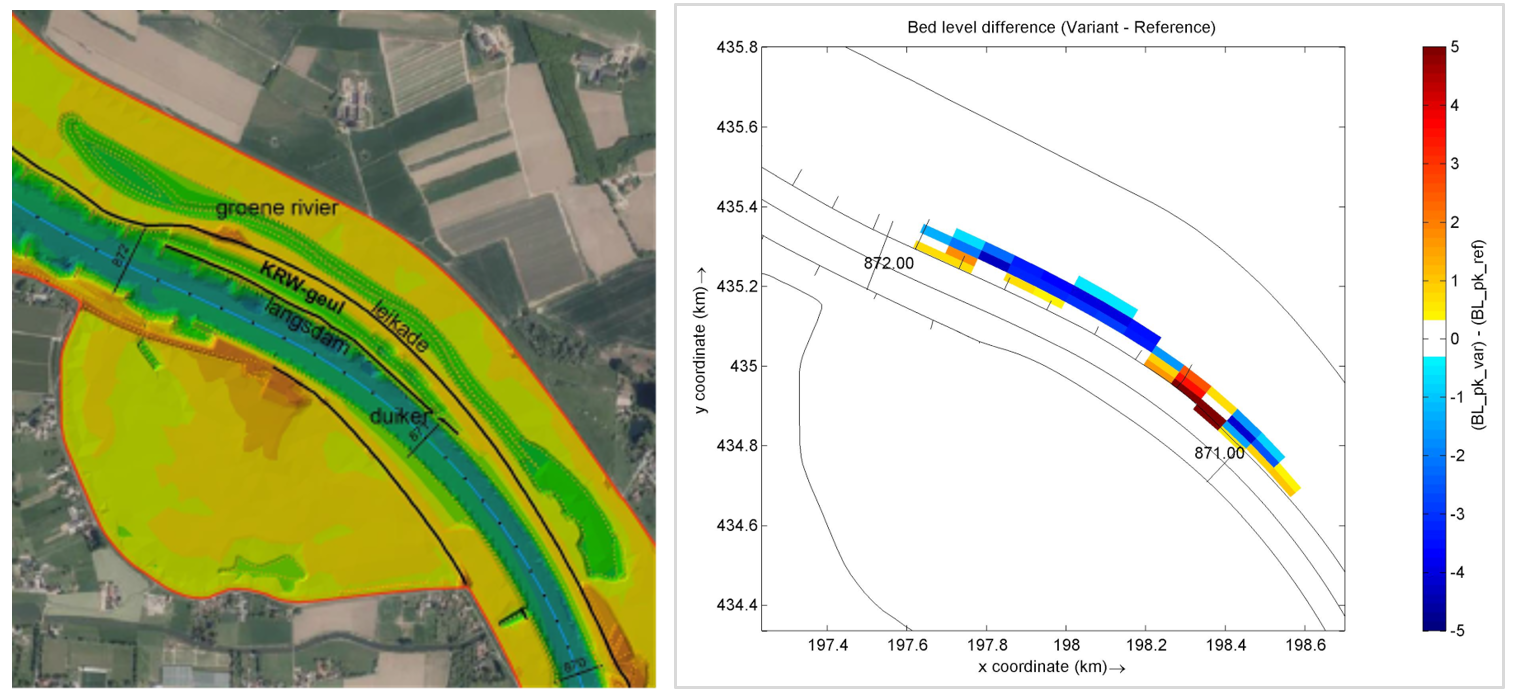
\includegraphics[width=\columnwidth]{figures/Pannerden_proj.png}
\caption{Side channel design (left) and initial representation on the grid (right).}
\label{Pannerden_proj}
\end{figure}

Since the intervention is located on the Rhine branches, the new \dfmi method requires the input of simulation results for 6 steady discharges: 1300, 2000, 3000, 4000, 6000, and \SI{8000}{\metre\cubed\per\second} at Lobith.
Contrary to Parlmerswaard case, the lowest discharge is relevant for this case.
Hence, \dfmi asks for the results of 12 simulations (6 discharges with and without intervention).

\citet{GiriJagers2022} observed that the morphological impact of this intervention was properly reproduced using a \dfmi analysis using the full set of discharges in the \emph{stepped-hydrograph} of the morphological simulation.
Here we compare the results with the results of the \dfmi analysis using the simplified hydrograph consisting of only the discharges 1300, 2000, 3000, 4000, 6000, and \SI{8000}{\metre\cubed\per\second} at Lobith.

\begin{figure}[b]
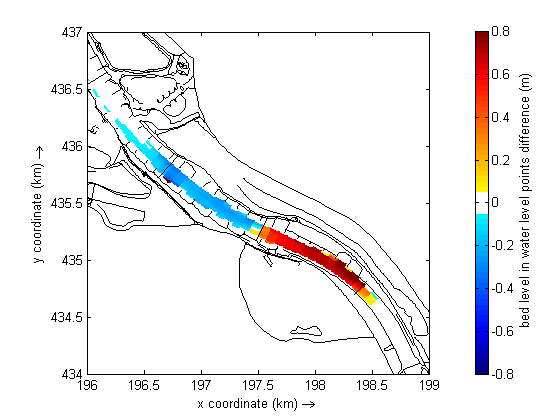
\includegraphics[width=\columnwidth/2]{figures/Pannerden_delft3d.png}
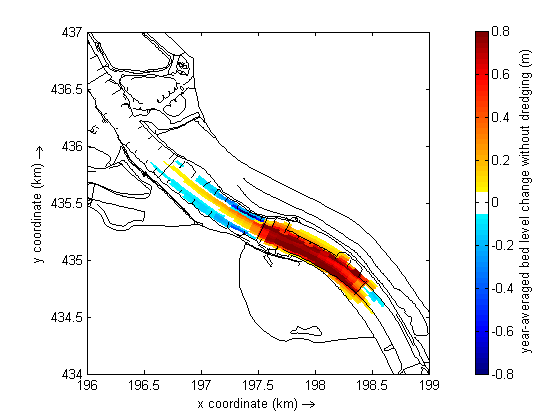
\includegraphics[width=\columnwidth/2]{figures/Pannerden_dfastmi.png}
%\fbox{\parbox{\columnwidth}{\todo{Results to be plotted side-by-side.}}}
\caption{Long-term morphological impact as obtained from a 12 year morphological simulation (left) and as obtained from \dfmi version 3 (right).
Visualized using QUICKPLOT.}
\label{Pannerden_mor}
\end{figure}

\autoref{Pannerden_mor} shows the results of a long-term (15 year) reference morphological simulation using Delft3D 4 (for details, see \citet{GiriJagers2022}) and the year-averaged equilibrium morphological impact as computed by \dfmi version 3.0.0.
The overall results match well although \dfmi suggests sedimentation in the centre of the channel downstream of the main sedimentation area whereas the morphological simulation doesn't show that behaviour.
This is a secondary effect compared to the primary impact.
The results are judged as valid.